%TCIDATA{LaTeXparent=0 0 sbrc_2013.tex}
%Review Method

\section{Método do Estudo}\label{sec:review_method}

Um mapeamento sistemático tem por objetivo classificar informações acerca de uma área de pesquisa de forma ampla e menos minuciosa que a tradicional revisão sistemática de estudos. Uma vez constatada a vasta quantidade de publicações no campo de SOC, escolheu-se esta metodologia para viabilizar a classifica\c c\~{a}o dos artigos. A metodologia adotada seguiu as diretrizes propostas em \cite{petersen:sms2008}, cujos passos necess\'{a}rios s\~{a}o descritos no restante desta se\c c\~{a}o.

\subsection{Protocolo do Estudo}

Um MS, assim como outras revisões literárias, estabelece o uso de um protocolo que documenta as etapas do mapeamento de modo a garantir sua replicação e diminuir possíveis erros por parte dos pesquisadores. Nele estão definidas as questões de pesquisa, os fóruns científicos onde as publicações s\~{a}o recuperadas, a \textit{string} de busca utilizada, os critérios de inclusão e exclusão de artigos, além das facetas de classificação.

\subsection{Quest\~{o}es de Pesquisa}\label{sec:questoesPesquisa}

As questões de pesquisa foram organizadas de acordo com a motivação desse estudo, que é investigar e categorizar as contribuições de pesquisa em Computação Orientada a Serviços no contexto de qualidade de serviço. Esse estudo tem como objetivo responder às seguintes perguntas: (1) \textbf{QP1} Quais áreas de SOC são mais frequentemente pesquisadas no contexto de qualidade de serviços? (2) \textbf{QP2} Quais atributos de qualidade são frequentemente considerados nos estudos abordados? (3) \textbf{QP3} Quais s\~{a}o os grupos de pesquisa mais ativo em SOC no contexto de QoS? (4) \textbf{QP4} Qual o foco da contribuição de pesquisa realizada?

A QP1 tem como objetivo trazer uma perspectiva do cen\'{a}rio das pesquisas em Computa\c{c}\~{a}o Orientada a Servi\c{c}os com foco em QoS atualmente. Para responder a essa pergunta, primeiramente definimos quais s\~{a}o as \'{a}reas que melhor caracterizam as diversas contribui\c{c}\~{o}es de pesquisa em SOC. Nota-se a importância da contribuição dada na definição dessa faceta, dada a escassez de referências que identifiquem as principais atividades envolvidas em SOC e que são alvos de pesquisa, tal qual a seleção, composição, monitoramento e adaptação de serviços, entre outras.

%Uma vez definidas essas \'{a}reas, realizamos ent\~{a}o a classifica\c{c}\~{a}o. 

Com rela\c{c}\~{a}o \`{a} QP2, pretendemos obter com esse estudo quais s\~{a}o os atributos de QoS mais frequentemente explorados em SOC. Em outras palavras, considerando que QoS, nesse contexto, envolve atributos como disponbilidade, confiabilidade, desempenho, seguran\c{c}a, escalabilidade, custo e SLA, quais desses atributos est\~{a}o de fato em foco. Com rela\c{c}\~{a}o \`{a} QP3, pretendemos tamb\'{e}m identificar quais s\~{a}o os grupos mais ativos no contexto desse estudo. Por fim, a QP4 almeja elucidar quais tipos de pesquisa s\~{a}o mais frequentes e inferir conclusões acerca da maturidade da pesquisa realizada na \'{a}rea. Vale ressaltar que no escopo deste artigo n\~{a}o pretendemos avaliar o m\'{e}rito dos trabalhos estudados.

% 	A QP1 almeja identificar o estado da pesquisa relacionada a SOC no contexto de qualidade de serviços em termos quantitativos, ou seja, apontar o número de publicações na área e os principais autores envolvidos. A QP2 busca mapear quais tópicos receberam maior atenção de pesquisa. Para isso, foram estabelecidas facetas de contribuição capazes de abranger relevantes atividades presentes no campo da computação orientada a serviços. A QP3 visa conhecer quais são, entre os atributos de qualidade de maior notoriedade, os que são com maior frequência contemplados. Além dos atributos de qualidade disponíveis, definiu-se dois outros itens de classificação de contexto. Um para representar a escolha genérica de atributos, isto é, contribuições que não definiram atributos específicos, e outro para representar atributos outros que não estejam definidos como itens de classificação de contexto. 

\subsection{Estratégia de Busca}\label{estrategia_busca}
%Our search strategy consisted of both manual and electronic search. Electronic search was performed in the following digital databases: ACM Digital Library, CiteSeerX, Compendex, Google Scholar, IEEE Xplore and SpringerLink. These are relevant electronic databases to computer science and software engineering, also used in a number of systematic studies in the area [2] .To formulate the search string for electronic database search, we used an approach suggested by Kitchenham [1]. The strategy derives the search string from the research questions using a composition with Boolean operators OR and AND. Table 1 presents the search string. The justification for using manual search was that creativity in RE is a relatively novel area, therefore manual search in conferences and journals provided extra confidence that relevant papers would be found.  To have a more representative set of studies, the “snow-balling" technique was adopted [3], in which the references of the identified papers were analyzed.
	Nossa estratégia de busca consistiu essencialmente na busca eletrônica nas seguintes bibliotecas digitais: 
\emph{ACM Digital Library, ScienceDirect, IEEE Xplore e SpringerLink}, que estão entre as bibliotecas mais relevantes para o contexto da nossa pesquisa. Para formular os termos de busca para a base de dados eletrônica, usamos a abordagem sugerida por Kitchenham~\cite{kitchenham:techReport2007,budgen:ppig2008}. A estrategia deriva os termos de busca a partir das questões de pesquisa usando uma composição com os operadores OR e AND. A  Tabela~\ref{tab:exTable1} apresenta a \texttt{string} de busca usada no nosso estudo. Para evitar a tendenciosidade sobre quais comunidades de pesquisa s\~{a}o as mais atuantes no nosso dom\'{i}nio de interesse, assim como obter um tamanho real do volume das contribuições, resolvemos não adotar técnicas como \emph{snow-balling} onde outros trabalhos relacionados podem ser encontrados a partir das referências dos trabalhos extraídos automaticamente \cite{budgen:ppig2008}.

%ganhamos um bom espaço sem usar items.. (Danilo)
%\begin{itemize}
%\item ACM Digital Library, 
%\item ScienceDirect, 
%\item IEEE Xplore, e 
%\item SpringerLink.
%\end{itemize} 

\begin{table}[ht]
\centering
\caption{Termos de Busca utilizados para pesquisa de publicações}
\label{tab:exTable1}
\begin{tabular}{p{0.75\linewidth}}
\hline
((``web service'' OR ``web services'' OR ``service oriented'' OR ``service-oriented'' OR SOA OR SaaS OR PaaS OR ``service orientation'' OR ``service-oriented computing'' OR ``service oriented computing'' OR SOC) AND (``quality of services'' OR ``quality of service'' OR QOS)) \\
\hline
\end{tabular}
\end{table}

Os termos \textit{SaaS} e\textit{PaaS} foram adicionados para representarem trabalhos mais recentes com foco na computação em nuvem, respectivamente definidos como Software como Service e Plataforma como Serviço. Entende-se que ambas abordagens fazem uso de conceitos e/ou tecnologias relacionados ao SOC, portanto foram incluídos no contexto desse estudo. 

\subsection{Crit\'{e}rio de Inclusão e Exclusão}\label{criterios_inc_exc}

Para filtrar os artigos coletados, utilizamos os seguintes critérios para inclus\~{a}o e exclus\~{a}o. Inclu\'{i}mos apenas artigos publicados em workshops, confer\^{e}ncias e peri\'{o}dicos nas bibliotecas digitais que satisfaziam nossa \texttt{string} de busca, conforme descrito na Se\c{c}\~{a}o \ref{estrategia_busca}. Artigos considerados como \emph{gray literature}, i.e. relat\'{o}rios t\'{e}cnicos e \emph{white papers} foram exclu\'{i}dos devido à grande quantidade de artigos científicos já considerados no escopo do mapeamento. No que tange \`{a}s contribui\c{c}\~{o}es em SOC, foram consideradas somente aquelas que lidavam com n\'{i}veis de abstra\c{c}\~{a}o acima do sistema operacional, e.g. relativas a middleware ou plataformas de distribui\c{c}\~{a}o. Contribui\c{c}\~{o}es que lidavam com SOC, mas que n\~{a}o tratavam de nenhum aspecto de QoS foram exclu\'{i}das. Tamb\'{e}m foram exclu\'{i}dos artigos que poderiam ser considerados como resumos estendidos, em geral, aqueles com n\'{u}mero de p\'{a}
ginas igual ou inferior a quatro. 

Por fim, o histograma da Figura~\ref{fig:barplotAnoPublicacoes} representa o número de publicações encontradas nas bibliotecas digitais consultadas, mostrando as primeiras ocorr\^{e}ncias em 2002. Percebemos que houve uma decaída no ano de 2011, porém a curva se mantém retorna sua tendência já em 2012. Com base nisso, resolvemos fazer uma avalia\c{c}\~{a}o que compreendesse um per\'{i}odo representativo para o mapeamento. Importante destacar que o ano de 2013 n\~{a}o foi considerado, pois at\'{e} o momento da coleta n\~{a}o era poss\'{i}vel obter informa\c{c}\~{o}es conclusivas sobre esse ano na data em que a classificação e análise dos demais anos foi executada.

\begin{figure*}[htb]
\centering
\includegraphics[scale=0.35]{imagens/histogram.png}
\caption{Quantidade de publica\c c\~{o}es relacionadas a QoS em SOC entre 2002 e 2012 coletadas}
\label{fig:barplotAnoPublicacoes}
\end{figure*}

\subsection{Coleta e Armazenamento dos Dados}

Inicialmente foram feitas consultas manuais em cada uma das bibliotecas digitais mencionadas na Se\c c\~{a}o~\ref{estrategia_busca}. Verificou-se ao todo um número de \AllPubs publicações a serem analisadas. Para atender a essa quantidade significativa de publica\c c\~{o}es, a coleta dos resultados de busca foi automatizada por um minerador capaz de recuperar as publica\c c\~{o}es nas bibliotecas digitais e armazenar as mesmas em um banco de dados. Mais especificamente, o minerador da Figura \ref{fig:system_architecture} armazena os metadados das publicações resultantes das buscas nas diferentes bibliotecas. 

%Descrever como o ambiente no Heroku está organizado (facets), explicar os termos principalmente os de Computação Orientada a Serviços qual a referência de significado que usamos. ``Each author individually extracted data from a subset of papers. We jointly  discussed unclear issues and solved discrepancies in the analysis.'' Os resultados tambem foram gerados automaticamente por meio da propria ferramenta....

\subsection{Ferramenta de Mapeamento Colaborativo}

Com base na experi\^{e}ncia de alguns dos autores deste artigo, que haviam observado a dificuldade em se trabalhar com revis\~{o}es sistem\'{a}ticas de forma colaborativa, decidiu-se pelo desenvolvimento de uma ferramenta de apoio para permitir a an\'{a}lise e classifica\c c\~{a}o dos artigos com maior eficiência e ubiquidade de trabalho, capaz também de gerar resultados gr\'{a}ficos em tempo real. Esta ferramenta consiste em um ambiente disponível em nuvem, com interfaces disponíveis para a listagem das publicações coletadas automaticamente pelo minerador ou de forma manual pela interface de registro de novas publicações. Sua arquitetura está representada na Figura \ref{fig:system_architecture}, com a seguinte descrição dos componentes:

\begin{itemize}

\item \textbf{Minerador:} Responsável pela coleta dos metadados das publicações a partir de uma determinada \textit{string} de busca. Para tanto, efetua requisições HTTP/REST a servidores web de bibliotecas digitais. Há duas possibilidades de retorno tratáveis para as chamadas dependendo da biblioteca usada: HTML puro representando a própria página de resultado de buscas ou em padrão XML, sendo ambos interpretados e tratados para a extração dos metadados. 

\item \textbf{Aplicação Web:} Consiste na aplicação que utiliza os dados coletados pelo minerador com funcionalidades de criação, edição, listagem e uso de usuários, grupos, facetas de classificação, publicações, revisões e geração síncrona de resultados. Sua implementação segue o modelo de desenvolvimento MVC com definições de entidades e relacionamentos genéricos para que o ambiente possa receber mapeamentos diversos que utilizem facetas de classificação criadas em tempo real. As Figuras \ref{fig:support_tool_02}, \ref{fig:support_tool_01} e \ref{fig:support_tool_03} ilustram, respectivamente, as interfaces de listagem e classificação de publicações e um exemplo de resultado gerado durante o mapeamento.

\item \textbf{Base de Dados:} Uma única base de dados como reposit\'{o}rio de coleta de dados do minerador e das classifica\c{c}\~{o}es e resultados obtidos por meio da aplicação web.

\end{itemize}

Também no ambiente da ferramenta de mapeamento, cada publicação pode ser classificada utilizando uma interface apropriada que contém os metadados do artigo, campos de observações e marcações dos itens de classificação definidos para o MS em questão, conforme Figura \ref{fig:support_tool_01}. O uso dessa ferramenta foi de grande importância para a viabilidade do MS diante da quantidade inicial de publicações coletadas. Al\'{e}m disso, tal ferramenta permitiu a realiza\c{c}\~{a}o do mapeamento de forma colaborativa onde os artigos s\~{a}o compartilhados entre diferentes grupos de usuários em suas respectivas sess\~{o}es autenticadas.

\begin{figure}[htb]
\centering
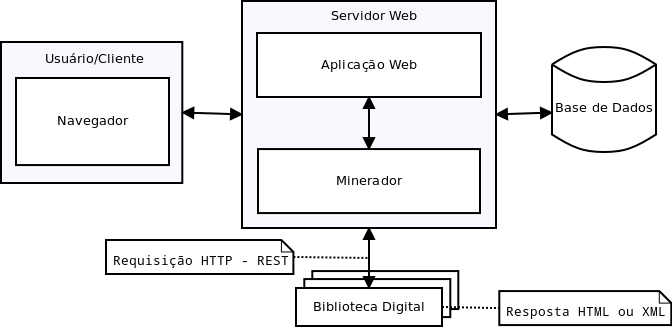
\includegraphics[scale=0.37]{figuras/system_architecture.png}
\caption{Arquitetura da Ferramenta de Mapeamento Colaborativo}
\label{fig:system_architecture}
\end{figure}

%\begin{figure}[h] 
%    \centering 
%    \subfigure[Listagem das publicações] 
%    { \label(Fig1){fig:support_tool_02} 
%      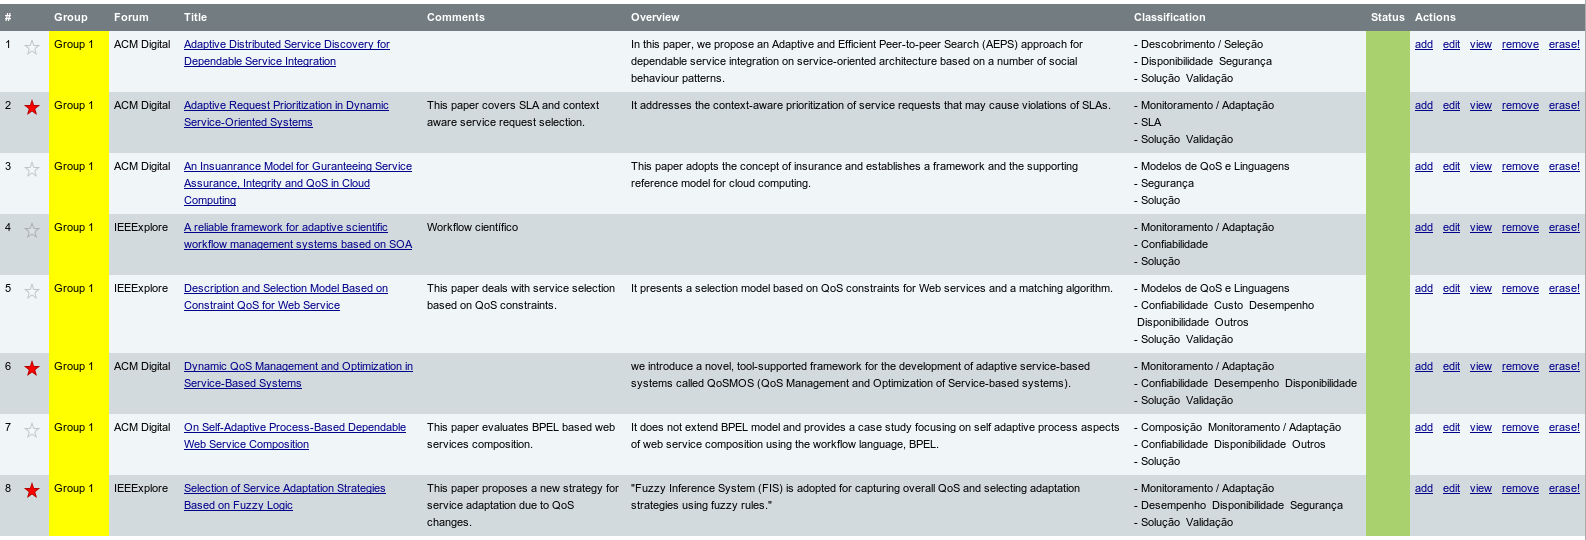
\includegraphics[scale=0.32]{figuras/Support_Tool_02.png} 
%    } \quad 
%    \subfigure[Interface usada para mapeamento] 
%    {\label(Fig2){fig:support_tool_01} 
%     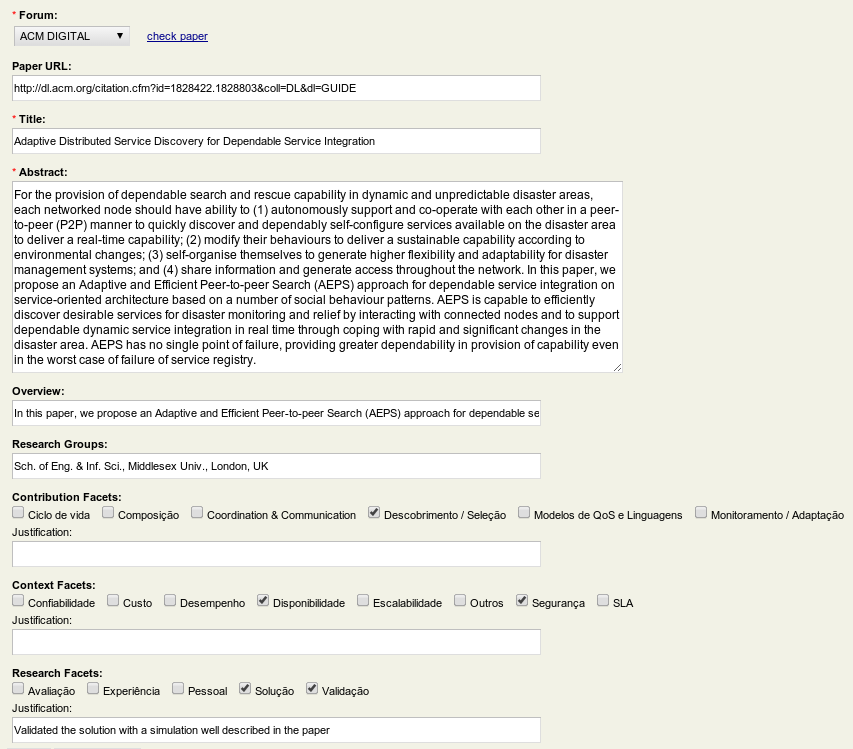
\includegraphics[scale=0.29]{figuras/Support_Tool_01.png}
%    }
%    \subfigure[Exemplo de resultado gerado para a faceta de QoS (contexto)] 
%    {\label(Fig2){fig:support_tool_03} 
%     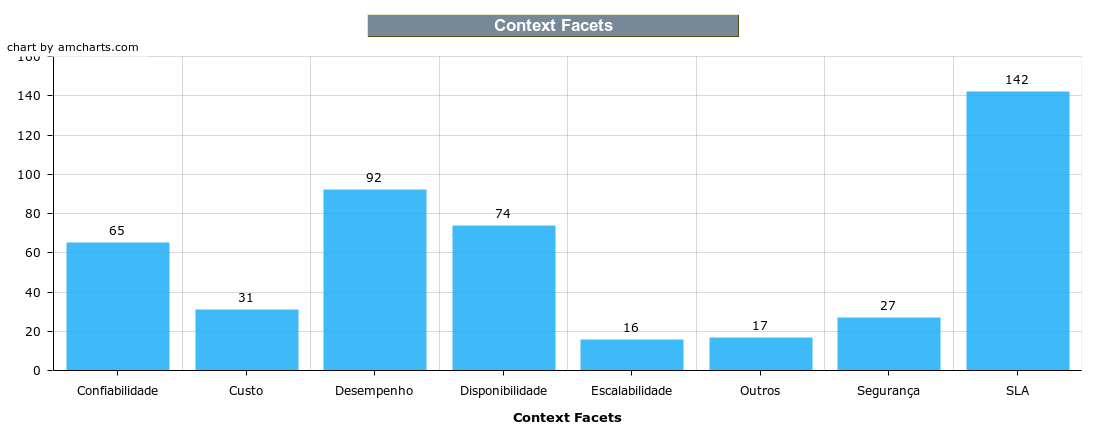
\includegraphics[scale=0.23]{figuras/Support_Tool_03.png} 
%    } 
%    \caption{Ferramenta de Mapeamento Colaborativo} 
%    \label{Fig:Implied} 
%\end{figure}

\begin{figure*}[htb]
\centering
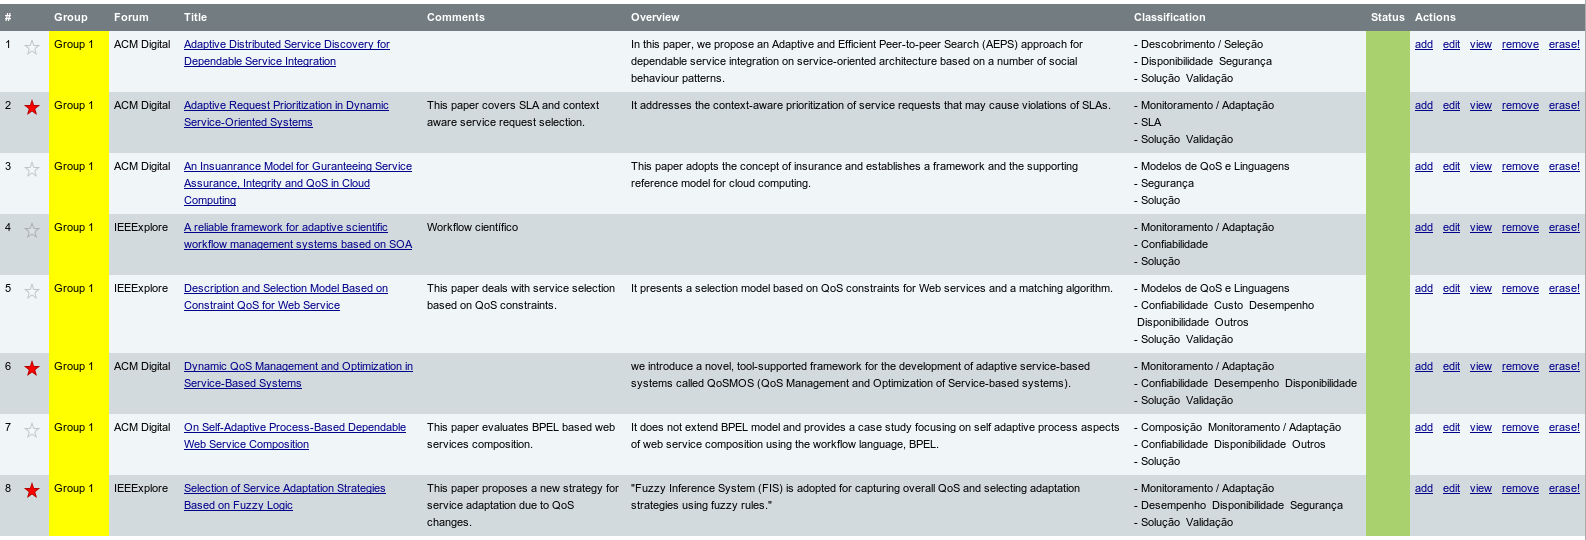
\includegraphics[scale=0.32]{figuras/Support_Tool_02.png}
\caption{Listagem das publicações}
\label{fig:support_tool_02}
\end{figure*}

\begin{figure}[htb]
\centering
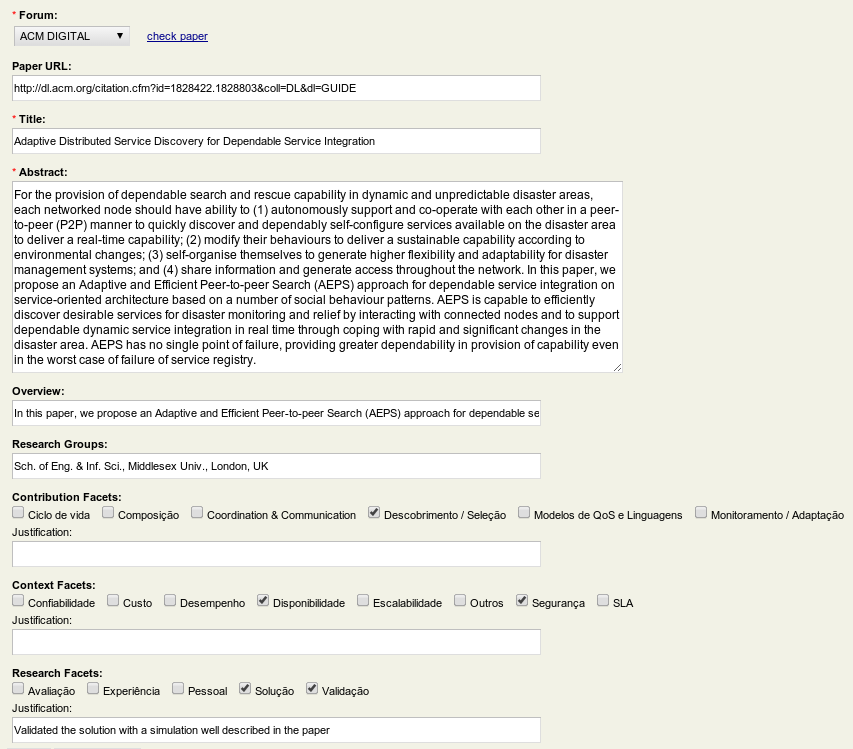
\includegraphics[scale=0.29]{figuras/Support_Tool_01.png}
\caption{Interface usada para mapeamento}
\label{fig:support_tool_01}
\end{figure}

\begin{figure}[htb]
\centering
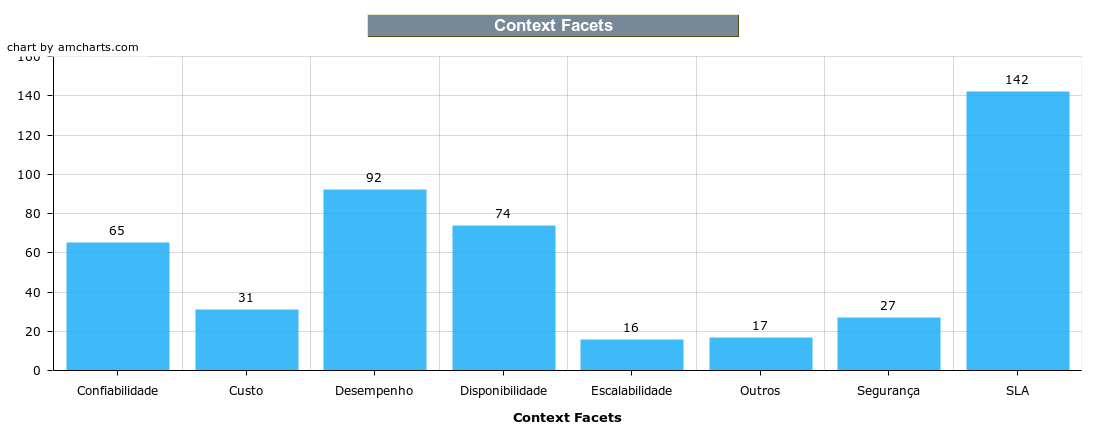
\includegraphics[scale=0.23]{figuras/Support_Tool_03.png}
\caption{Exemplo de resultado gerado para a faceta de QoS (contexto)}
\label{fig:support_tool_03}
\end{figure}

A partir da distribuição automática de artigos para cada um dos pesquisadores pela aplicação web, foram excluídas manualmente as publicações que não se adequaram aos critérios definidos na Seção \ref{criterios_inc_exc}, resultando em uma lista final de \AcceptedPubs artigos. Portanto, da quantidade inicial coletada nas bases de busca, 75\% foram considerados fora dos critérios adotados para o mapeamento. Tal processo, assim como a classificação, foram realizados manualmente e individualmente, tendo havido frequente discussão para eliminar quaisquer dúvidas e inconsistências de interpretações quanto aos critérios de inclusão, exclusão e facetas de classificação. 

\subsection{Facetas de Classificação}

Os artigos foram classificados de acordo com as categorias:
\begin{itemize}
\item[-] \textbf{Contribuição}: Essa faceta classifca partes relevantes de SOC, de modo a agrupar trabalhos de pesquisa por subáreas de contribuição. Definir essa faceta foi um primeiro desafio para o grupo, pois n\~{a}o encontramos na literatura algum trabalho que defina de forma clara e concisa as dimensões que devem definir e constituir SOC. Considerando a experi\^{e}ncia dos autores e depois de um vasto estudo da literatura, os autores definiram os seguintes atributos dessa faceta: \emph{composição, coordenação \& comunicação, descoberta \& seleção, ciclo de vida, monitoramento \& adaptação} e  \emph{modelos de QoS \& linguagens}. Algumas categorias que haviam uma forte correla\c{c}\~{a}o foram classificadas em um grupo, como  \emph{monitoramento \& adaptação} e \emph{coordenação \& comunicação}. Em particular, a categoria \emph{modelos de QoS \& linguagens} engloba publicações que definem extensões ou novos modelos de QoS por meio de modelos computacionais, linguagens, especificações e/ou ontologias a 
serem utilizadas em sistemas baseados em serviços para o suporte à analise, garantia ou gerenciamento de QoS.

\item[-] \textbf{Contexto}: Essa faceta representa os atributos de qualidade de maior relevância para SOC, além das opções para os demais atributos não mencionados, atributos genéricos e referentes à SLA. São eles: \emph{disponibilidade, desempenho, confiabilidade, escalabilidade, segurança, custo, outros} e \emph{SLA}. O item SLA engloba trabalhos que não especificam quais atributos de qualidade em específico estão tratando, sendo consideradas contribuições genéricas no contexto de QoS. 

\item[-] \textbf{Pesquisa}: A última faceta \'{e} usada para caracterizar o tipo de pesquisa realizada. Para definir essa faceta, utilizamos as defini\c{c}\~{o}es em~\cite{Wieringa:10.1007/s00766-005-0021-6}: 
\emph{solu\c c\~{a}o} (artigos que propõem uma nova solução e que, ocasionalmente, utilizam um pequeno exemplo para verificarem a sua viabilidade), \emph{validação} (artigos que apresentam 
estudos empíricos ou provas que corroboram a aplicabilidade de alguma t\'{e}cnica), \emph{avalia\c c\~{a}o} (artigos que apresentam 
algum tipo de avalia\c c\~{a}o comparativa entre t\'{e}cnicas propostas e/ou existentes e discorrem sobre os benefícios e limitações num contexto em que já houve casos de uso reais) e \emph{experiência pessoal} (quando os autores apresentam a exper\^{e}ncia pr\'{a}tica do uso de alguma t\'{e}cnica ou discutem tend\^{e}ncias de pesquisa sobre um tema espec\'{i}fico).
\end{itemize}

%Artigos classificados em avalia\c{c}\~{a}o s\~{a}o aqueles que .... Enquanto que os artigos avaliados em valida\c{c}\~{a}o s\~{a}o aqueles que .... No entanto, vale ressaltar que artigos classificados como solu\c{c}\~{a}o podem tamb\'{e}m ser mapeados como valida\c{c}\~{a}o ou avalia\c{c}\~{a}o, caso estas fa\c{c}am parte da contribui\c{c}\~{a}o do trabalho estudado.

%\begin{itemize}
%\item {\bf Composição} Trata da agregação de serviços visando o estabelecimento de novas aplicações ou seu rearranjo de forma a manter determinados níveis de QoS pré-estabelecidos ou acordados.
%\item {\bf Coordenação e Comunicação} Trata da orquestração de serviços para atender a um objetivo determinado num período de duração correspondente à atividade executada. Além disso, envolve a troca de mensagens através do orquestrador, portanto também envolve protocolos específicos para a transação e comunicação em geral.
%\item {\bf Descoberta e Seleção} Refere-se à publicação, descoberta e seleção de serviços em registros públicos ou privados considerando aspectos de qualidade de serviços.
%\item {\bf Ciclo de vida} Refere-se às fases da engenharia de software dentro do domínio de sistemas baseados em serviços, tal qual projeto, desenvolvimento, manutenção e testes.
%\item {\bf Monitoramento e Adaptação} Relacionados ao tempo de execução, monitoramento de atributos não funcionais e adaptação de configuração e disposição de serviços visando manter os níveis desejados de QoS.
%\item {\bf Modelos de QoS e Linguagens} Engloba publicações que definem extensões ou novos modelos de QoS por meio de linguagens, especificações e ontologias a serem utilizadas em sistemas baseados em serviços e na definição de contratos de serviços que incluam garantias de QoS.
%\end{itemize} 